\documentclass[conference,a4paper]{IEEEtran}
\IEEEoverridecommandlockouts
% The preceding line is only needed to identify funding in the first footnote. If that is unneeded, please comment it out.
%Template version as of 6/27/2024

\usepackage{cite}
\usepackage{amsmath,amssymb,amsfonts}
\usepackage{algorithmic}
\usepackage{graphicx}
\usepackage{textcomp}
\usepackage{xcolor}
\usepackage{booktabs}
\usepackage{url}
\usepackage[hidelinks]{hyperref}
\def\BibTeX{{\rm B\kern-.05em{\sc i\kern-.025em b}\kern-.08em
    T\kern-.1667em\lower.7ex\hbox{E}\kern-.125emX}}
\begin{document}

\title{Assignment 1 : Sphere Neural Network %\\
%{\footnotesize \textsuperscript{*}Note: Sub-titles are not captured for https://ieeexplore.ieee.org  and
%should not be used}
%\thanks{Identify applicable funding agency here. If none, delete this.}
}

\author{\IEEEauthorblockN{Renjiro Owen}
\textit{Victoria University Wellington}\\
Wellington, New Zealand\\
owenrenj@myvuw.ac.nz}
\graphicspath{{../../}}
\maketitle

\section{Introduction}

Generative models learn to generate samples that resemble a desired probability distribution. In this assignment, fully connected neural networks are trained to learn transformations between distributions using explicit stochastic gradient descent (SGD) iterations.

First, a network $f_1$ maps a two-dimensional Gaussian distribution $Z \sim \mathcal{N}(0,I)$ to a two-dimensional uniform distribution over a unit square. A second network $f_2$ learns the inverse mapping from the uniform distribution back to a Gaussian distribution. The effect of $L_1$ and $L_2$ weight regularisation is also investigated by examining how regularisation changes the network weights and generated distribution.

Finally, a third network $f_3$ maps a one-dimensional uniform input to a two-dimensional Gaussian distribution. This demonstrates how a nonlinear neural network can learn a mapping from a lower-dimensional input to samples that approximate a higher-dimensional distribution.

\section{Theory}

A generative model learns to produce samples that follow a desired probability distribution. A common approach is to learn a transformation from a simple source distribution, such as a Gaussian, to a target distribution using a neural network \cite{goodfellow2016}. In this work, the neural network represents a function $f_\theta$ whose parameters $\theta$ are learned from samples of the source and target distributions.

The networks are trained using stochastic gradient descent (SGD). At each iteration, a minibatch of samples is generated, a loss measuring the difference between the generated and desired distributions is calculated, and the network parameters are updated according to

\begin{equation}
	\theta \leftarrow \theta - \eta \nabla_\theta L,
\end{equation}

where $\eta$ is the learning rate and $L$ is the training loss. SGD is widely used for training neural networks because it provides an efficient approximation of the gradient using batches of samples \cite{goodfellow2016}.

Regularisation can be used to control the size of neural network weights and reduce model complexity. In this work, both $L_1$ and $L_2$ regularisation are considered. $L_1$ regularisation penalises the absolute values of the weights, while $L_2$ regularisation penalises their squared values \cite{goodfellow2016}.

The $L_1$ regularisation term is defined as

\[
\Omega_{L_1}(w) = |w|_1 = \sum_i |w_i|.
\]

The $L_2$ regularisation term is defined as

\[
\Omega_{L_2}(w) = \frac{1}{2}|w|_2^2
= \frac{1}{2}\sum_i w_i^2.
\]

The regularised loss used for training can therefore be written as
\[
L_{\mathrm{MMD}}
+
\lambda_1 \Omega_{L_1}(w)
+
\lambda_2 \Omega_{L_2}(w),
\]

where $L_{\mathrm{MMD}}$ measures the difference between the generated and target distributions, while $\lambda_1$ and $\lambda_2$ control the strength of the $L_1$ and $L_2$ penalties, respectively. $L_1$ regularisation can encourage sparse weights, whereas $L_2$ regularisation encourages weights to remain small \cite{goodfellow2016}.


\section{Experiments}

\subsection{Experimental Setup}
\subsubsection{F1}
The $f_1$ generator uses a fully connected neural network with two hidden layers of 64 neurons and ReLU activations, followed by a Sigmoid output layer. It maps $z\sim\mathcal{N}(0,I)$ to two-dimensional samples in $[0,1]^2$.

Training used a batch size of 256, learning rate of (0.01), and 5,000 iterations. The MMD loss with a Gaussian kernel $\sigma=0.1$ was used to measure the difference between generated samples and samples from $U([0,1]^2)$. After calculating the MMD loss, gradients were obtained through backpropagation and each network parameter was updated according to
\[
\theta \leftarrow \theta-\eta\nabla_{\theta}\mathcal{L}_{\mathrm{MMD}},
\]
The MMD loss was recorded at every iteration to monitor the training process.
\subsubsection{F2}

The $f_2$ generator uses a fully connected neural network with three hidden layers of 64 neurons using Tanh activations, followed by a two-dimensional linear output layer. The model maps $z\sim U([0,1]^2)$ to the target distribution $\mathcal{N}(0,I)$.

Training used a batch size of 512, learning rate of (0.01), and 10,000 iterations. The MMD loss with a Gaussian kernel $(\sigma=0.1)$ was used to compare the generated and target distributions. Parameters were updated using explicit SGD.
\subsubsection{L1 L2}

The $f_1$ architecture was extended with L1 and L2 regularisation to investigate their effects on generator training. The batch size, learning rate, and number of iterations were kept at 256, $0.01$, and 5,000, respectively. The total loss was defined as the MMD loss plus weighted L1 and L2 penalties.

Experiments were conducted using $\lambda=0.001$, $0.005$, and $0.01$ individually for L1 and L2 regularisation. Additional experiments applied both L1 and L2 simultaneously using $\lambda=0.001$ and $0.01$. This allowed the individual and combined effects of the regularisation terms on the generated distribution to be compared.

\subsubsection{f3}

The \(f_3\) generator uses a one-dimensional input \(y\sim U([0,1])\), which is transformed into nonlinear Fourier features using sine and cosine functions. The number of features was varied between 4, 8, and 16 to investigate the effect of feature complexity on the generated distribution. These features are passed through two fully connected hidden layers of 64 neurons with Tanh activations, followed by a two-dimensional linear output layer. The model maps the one-dimensional uniform input to the target distribution \(\mathcal{N}(0,I)\).

For each feature configuration, training used a batch size of 512, learning rate of \(0.01\), and 5,000 iterations. The MMD loss with a Gaussian kernel (\(\sigma=0.1\)) was used to compare the generated samples with samples from the target distribution. Parameters were updated using explicit SGD.

\subsection{Test Performance}
\subsubsection{f1}
The \(f_1\) generator was trained for 5,000 iterations using a learning rate of \(0.01\) and a batch size of 256. The MMD loss decreased substantially from \(0.851574\) at the start of training to \(0.005059\) at iteration 4,500. Although some fluctuations occurred during training, the overall trend shows that the generator successfully learned the target distribution.

The generated samples were then compared visually with the target distribution. As shown in Figure~\ref{fig:target_gen_f1}, the generated distribution is very similar to the target \(U([0,1]^2)\), with only small random variations. This indicates that \(f_1\) was able to effectively approximate the target distribution.

\subsubsection{f2}
The \(f_2\) generator was trained for 10,000 iterations using a learning rate of \(0.01\) and a batch size of 512. The MMD loss decreased substantially from \(0.931694\) at the start of training to approximately \(0.005\) during the later stages. Although the loss fluctuated slightly throughout training, it remained relatively low, indicating that the generated distribution became closer to the target distribution.

However, as shown in Figure~\ref{fig:target_gen_f2}, the generated samples form a diamond-shaped distribution concentrated around the centre of the target Gaussian distribution. While the generator successfully learned the approximate central location of the target, it did not reproduce the Gaussian shape and spread accurately. This suggests that a low MMD loss does not necessarily mean that the generated distribution visually matches the target distribution.
\subsubsection{L1 and L2 Regularisation}

The effect of increasing L1 regularisation can be observed by comparing Figures~\ref{fig:genf1_l1_001}, \ref{fig:genf1_l1_005}, and \ref{fig:genf1_l1_01}. As the L1 coefficient increases from \(0.001\) to \(0.01\), the distributions on the left and bottom right are progressively pushed towards the centre. This causes these regions to become slightly denser, while reducing the spread of the generated samples.

The effect of L2 regularisation is shown in Figures~\ref{fig:genf1_l2_001}, \ref{fig:genf1_l2_005}, and \ref{fig:genf1_l2_01}. Increasing the L2 coefficient mainly reduces the overall range of the generated distribution. The samples become more concentrated towards the centre, resulting in a smaller overall spread.

When L1 and L2 are applied together, as shown in Figures~\ref{fig:genf1_l1l2_001} and \ref{fig:genf1_l1l2_01}, the effects of both regularisation terms become more apparent. The distribution shrinks towards the centre while the left and top regions become denser. Overall, stronger combined regularisation produces a more concentrated distribution with reduced spread and increased density in these regions.

\subsubsection{f3}

The effect of increasing the number of nonlinear features can be seen in Figures~\ref{fig:target_gen_f3_4}, \ref{fig:target_gen_f3_8}, and \ref{fig:target_gen_f3_16}. With 4 features, the generated samples form a V-shaped curve. Increasing the features to 8 produces a more curved distribution. With 16 features, the generated samples become more complex, circling around the centre multiple times. This shows that increasing the number of nonlinear features gives the generator greater flexibility to produce more complex patterns.

The loss results also show that the MMD loss generally decreases as more features are added. This indicates that increasing the number of features improves the generator's ability to match the target distribution according to the MMD metric, although the generated shape does not necessarily become more visually similar to the target Gaussian.
\section{Conclusion}

This study investigated neural network generators for learning target distributions using MMD. The \(f_1\) generator successfully learned the uniform distribution, producing samples very similar to the target. In contrast, \(f_2\) achieved a low MMD loss but produced a diamond-shaped distribution rather than accurately reproducing the Gaussian shape, showing that a low MMD does not always indicate a good visual match.

The \(f_3\) experiments showed that increasing the number of nonlinear features allowed the generator to produce increasingly complex patterns, while generally reducing the MMD loss. L1 and L2 regularisation also affected the generated distributions by increasing concentration and reducing their overall range. Overall, the results demonstrate that architecture, feature complexity, and regularisation have an important effect on the quality of generated distributions.


\newpage
\section{Statement}

\textbf{Tools Used}
\begin{itemize}
	\item Python 3
	\item Google Colab
	\item PyTorch
	\item Matplotlib
	\item ChatGPT \cite{chatgpt2026} (used for proofreading and improving the report wording)
\end{itemize}

I declare that this assignment is my own work. The implementation, experimentation, model training, and evaluation were completed by me. Artificial intelligence tools were used only for language assistance during the preparation of this report.

\textbf{Google Colab Code}

\href{https://drive.google.com/file/d/1udU5_BWTRcC0YNPkJpVkKqKHk0itPn2L/view?usp=sharing}
{Google Drive link}

\bibliographystyle{IEEEtran}   % or plain, unsrt, apalike, etc.
\bibliography{references}

\section*{Appendix}

\begin{figure}[ht]
	\centering
	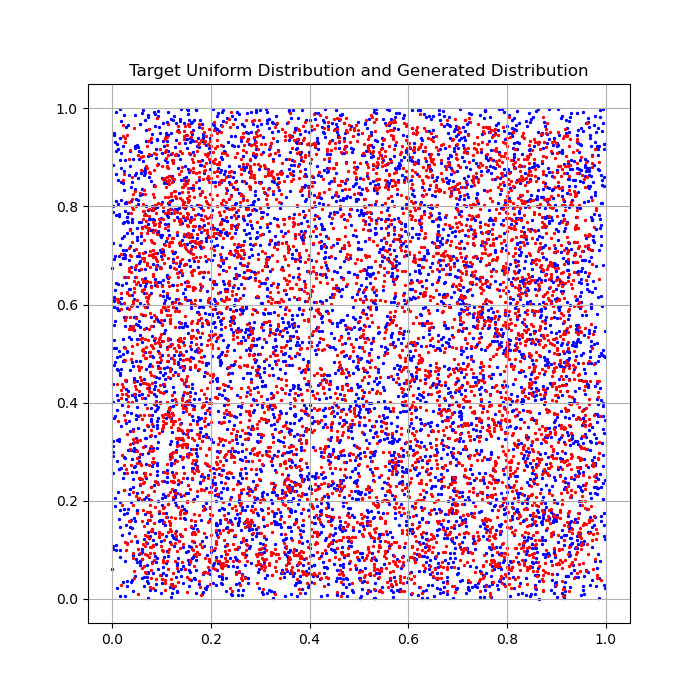
\includegraphics[width=0.8\linewidth]{targetVSgenf1.png}
	\caption{Comparison between the target distribution and the generated distribution for $f_1$.}
	\label{fig:target_gen_f1}
\end{figure}
\begin{figure}[ht]
	\centering
	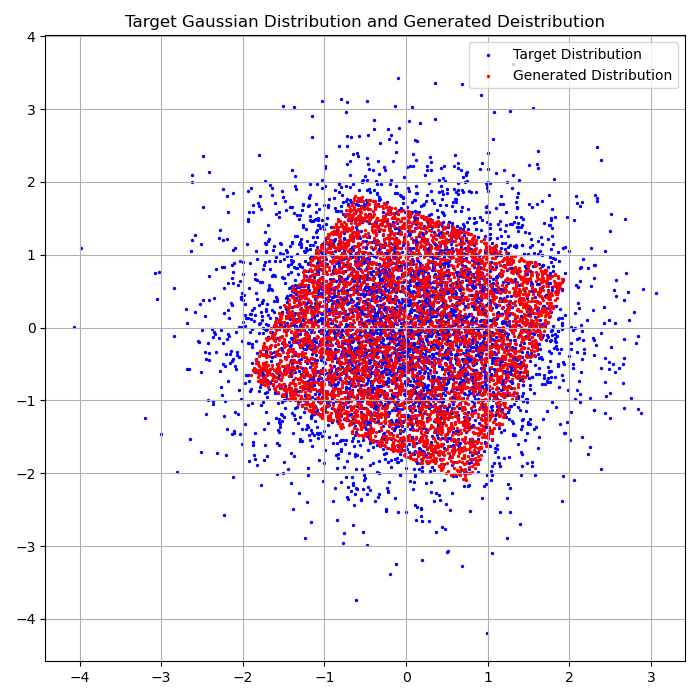
\includegraphics[width=0.8\linewidth]{targetVSgenf2.png}
	\caption{Comparison between the target distribution and the generated distribution for $f_2$.}
	\label{fig:target_gen_f2}
\end{figure}

\begin{figure}[ht]
	\centering
	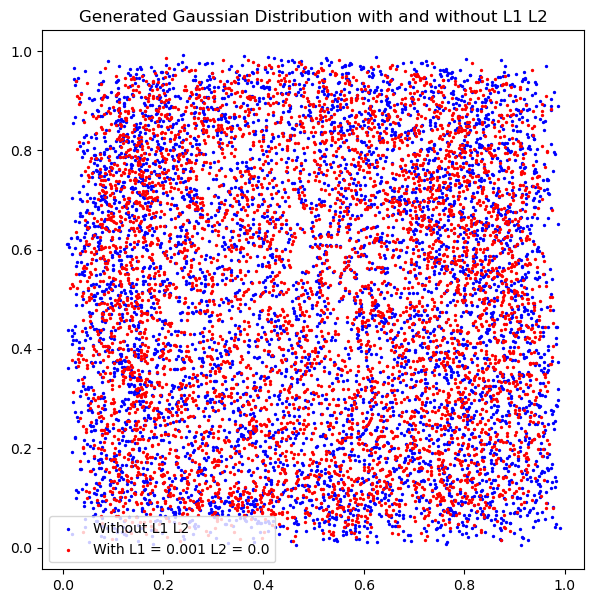
\includegraphics[width=0.8\linewidth]{genf1L10.001L20.0.png}
	\caption{Generated distribution for $f_1$ using L1 regularisation with $\lambda_{L1}=0.001$.}
	\label{fig:genf1_l1_001}
\end{figure}

\begin{figure}[ht]
	\centering
	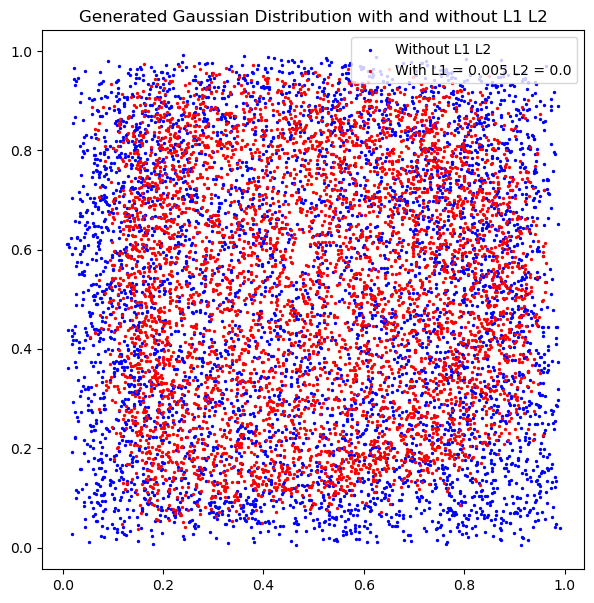
\includegraphics[width=0.8\linewidth]{genf1L10.005L20.0.png}
	\caption{Generated distribution for $f_1$ using L1 regularisation with $\lambda_{L1}=0.005$.}
	\label{fig:genf1_l1_005}
\end{figure}

\begin{figure}[ht]
	\centering
	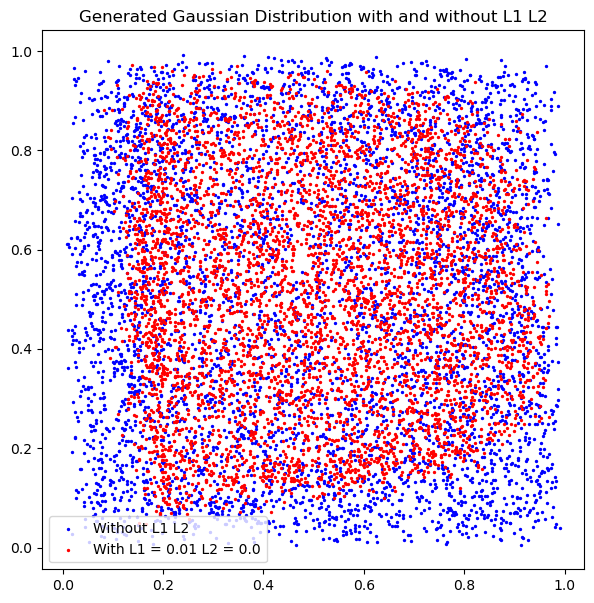
\includegraphics[width=0.8\linewidth]{genf1L10.01L20.0.png}
	\caption{Generated distribution for $f_1$ using L1 regularisation with $\lambda_{L1}=0.01$.}
	\label{fig:genf1_l1_01}
\end{figure}

\begin{figure}[ht]
	\centering
	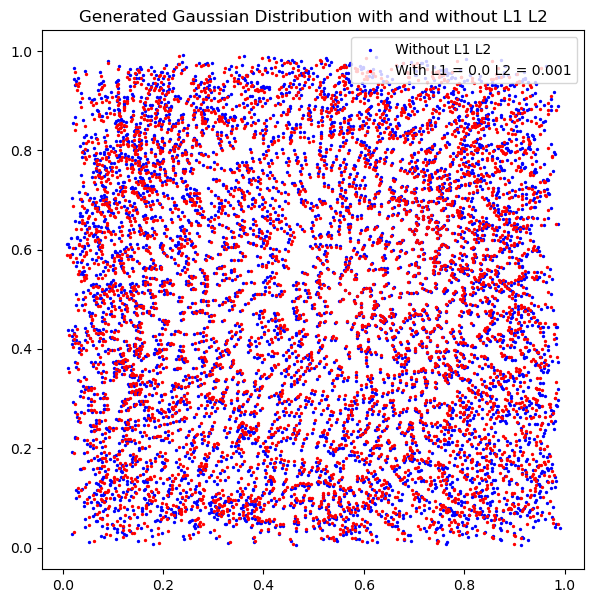
\includegraphics[width=0.8\linewidth]{genf1L10.0L20.001.png}
	\caption{Generated distribution for $f_1$ using L2 regularisation with $\lambda_{L2}=0.001$.}
	\label{fig:genf1_l2_001}
\end{figure}

\begin{figure}[ht]
	\centering
	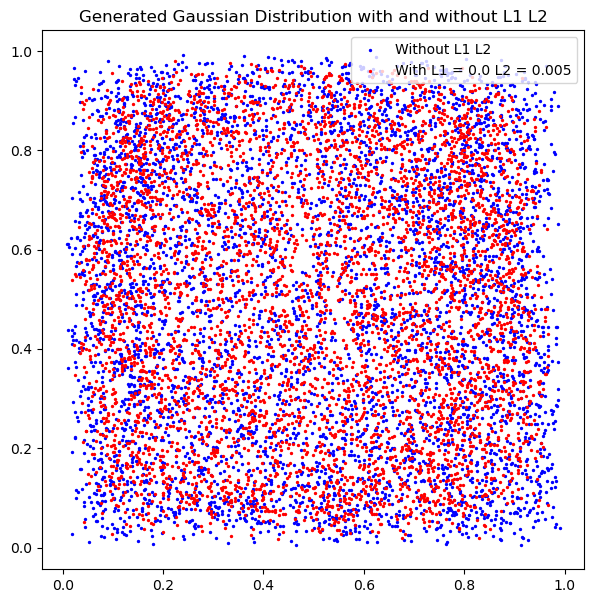
\includegraphics[width=0.8\linewidth]{genf1L10.0L20.005.png}
	\caption{Generated distribution for $f_1$ using L2 regularisation with $\lambda_{L2}=0.005$.}
	\label{fig:genf1_l2_005}
\end{figure}

\begin{figure}[ht]
	\centering
	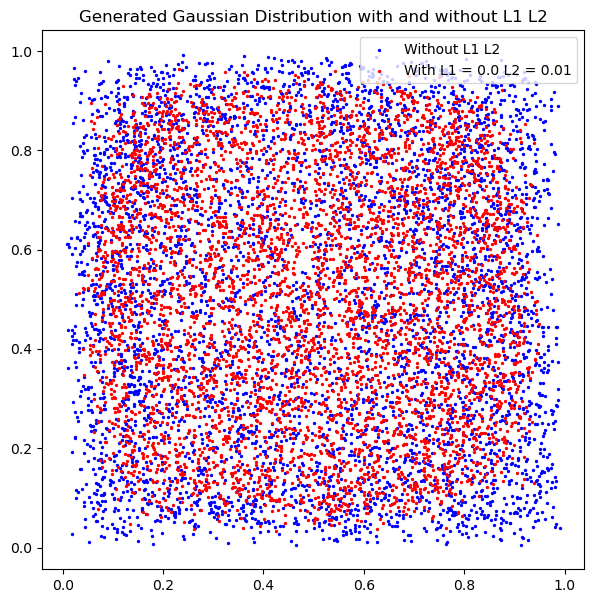
\includegraphics[width=0.8\linewidth]{genf1L10.0L20.01.png}
	\caption{Generated distribution for $f_1$ using L2 regularisation with $\lambda_{L2}=0.01$.}
	\label{fig:genf1_l2_01}
\end{figure}

\begin{figure}[ht]
	\centering
	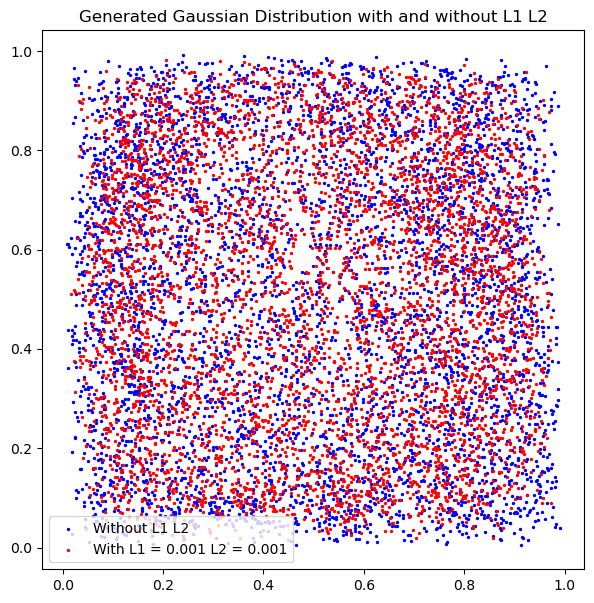
\includegraphics[width=0.8\linewidth]{genf1L10.001L20.001.png}
	\caption{Generated distribution for $f_1$ using both L1 and L2 regularisation with $\lambda_{L1}=\lambda_{L2}=0.001$.}
	\label{fig:genf1_l1l2_001}
\end{figure}

\begin{figure}[ht]
	\centering
	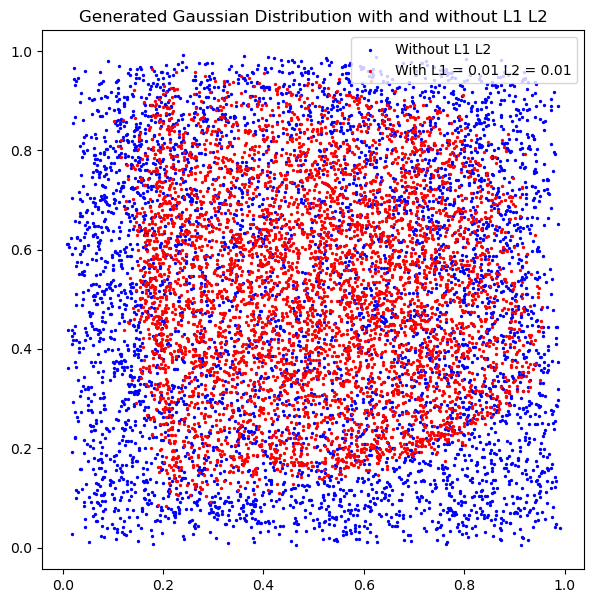
\includegraphics[width=0.8\linewidth]{genf1L10.01L20.01.png}
	\caption{Generated distribution for $f_1$ using both L1 and L2 regularisation with $\lambda_{L1}=\lambda_{L2}=0.01$.}
	\label{fig:genf1_l1l2_01}
\end{figure}

\begin{figure}[ht]
	\centering
	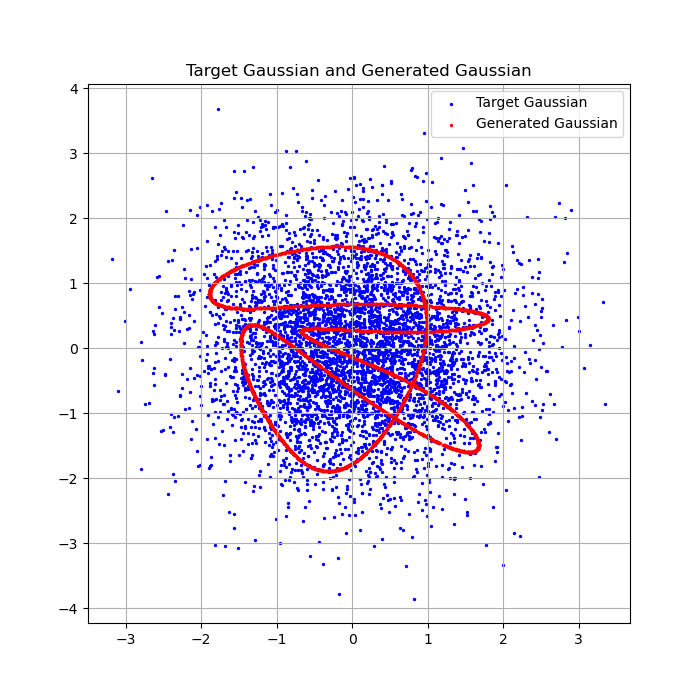
\includegraphics[width=0.8\linewidth]{targetVSgenf34features.png}
	\caption{Generated distribution for $f_3$ using 4 nonlinear features compared with the target distribution.}
	\label{fig:target_gen_f3_4}
\end{figure}
\begin{figure}[ht]
	\centering
	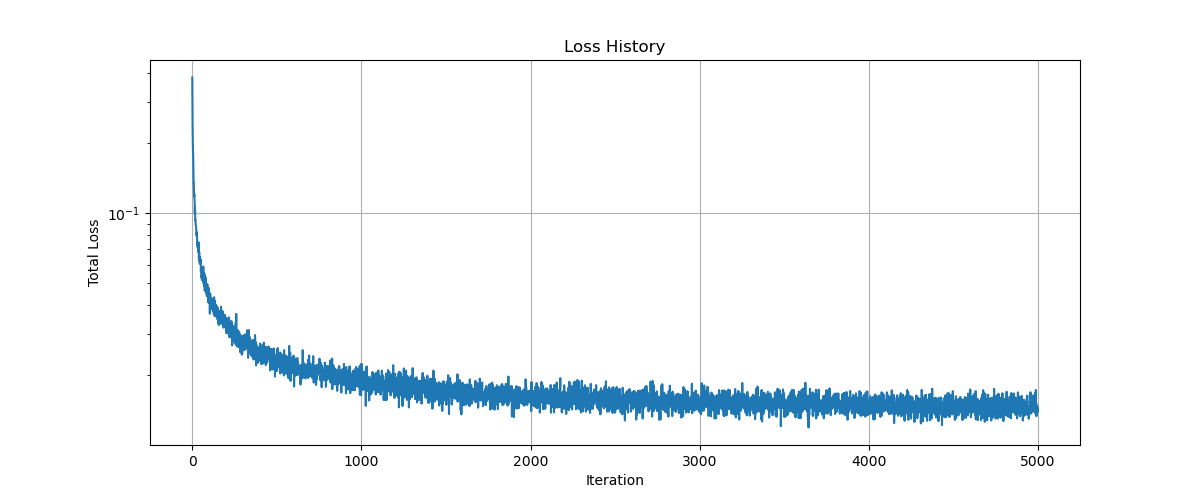
\includegraphics[width=0.8\linewidth]{lossgenf34features.png}
	\caption{Training loss for the generator with 4 nonlinear features.}
	\label{fig:loss_f3_4}
\end{figure}
\begin{figure}[ht]
	\centering
	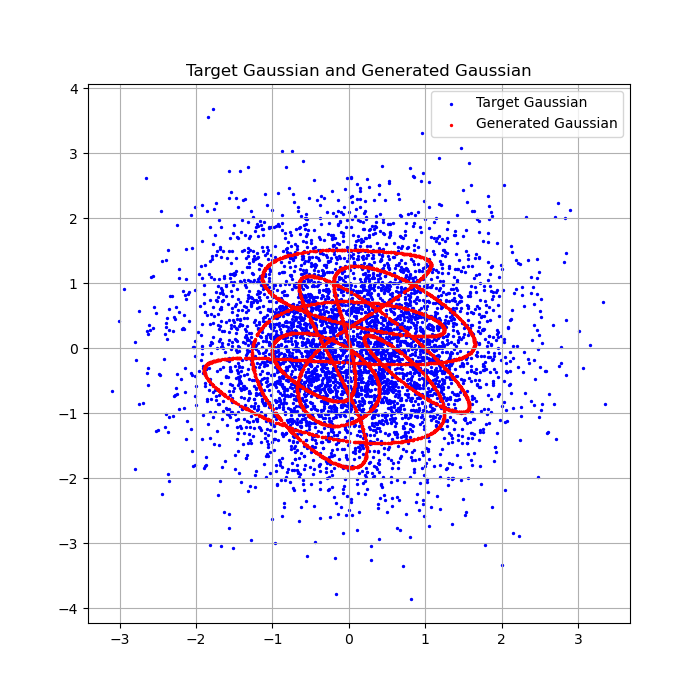
\includegraphics[width=0.8\linewidth]{targetVSgenf38features.png}
	\caption{Generated distribution for $f_3$ using 8 nonlinear features compared with the target distribution.}
	\label{fig:target_gen_f3_8}
\end{figure}
\begin{figure}[ht]
	\centering
	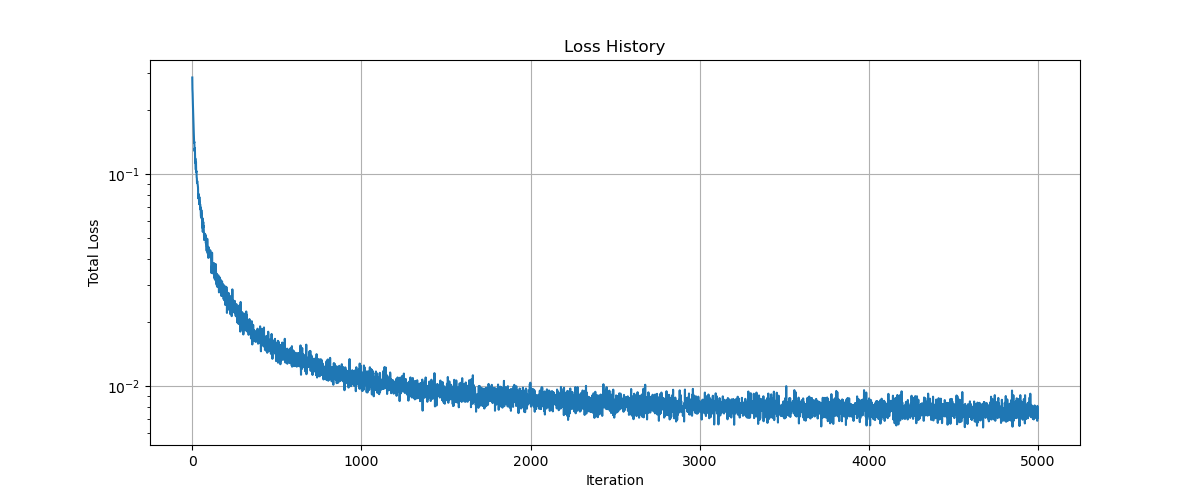
\includegraphics[width=0.8\linewidth]{lossgenf38features.png}
	\caption{Training loss for the generator with 8 nonlinear features.}
	\label{fig:loss_f3_8}
\end{figure}
\begin{figure}[ht]
	\centering
	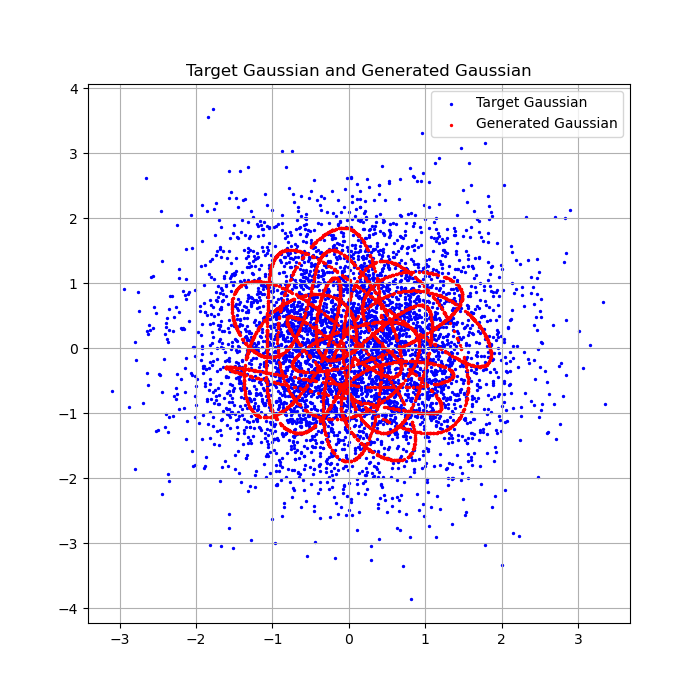
\includegraphics[width=0.8\linewidth]{targetVSgenf316features.png}
	\caption{Generated distribution for $f_3$ using 16 nonlinear features compared with the target distribution.}
	\label{fig:target_gen_f3_16}
\end{figure}
\begin{figure}[ht]
	\centering
	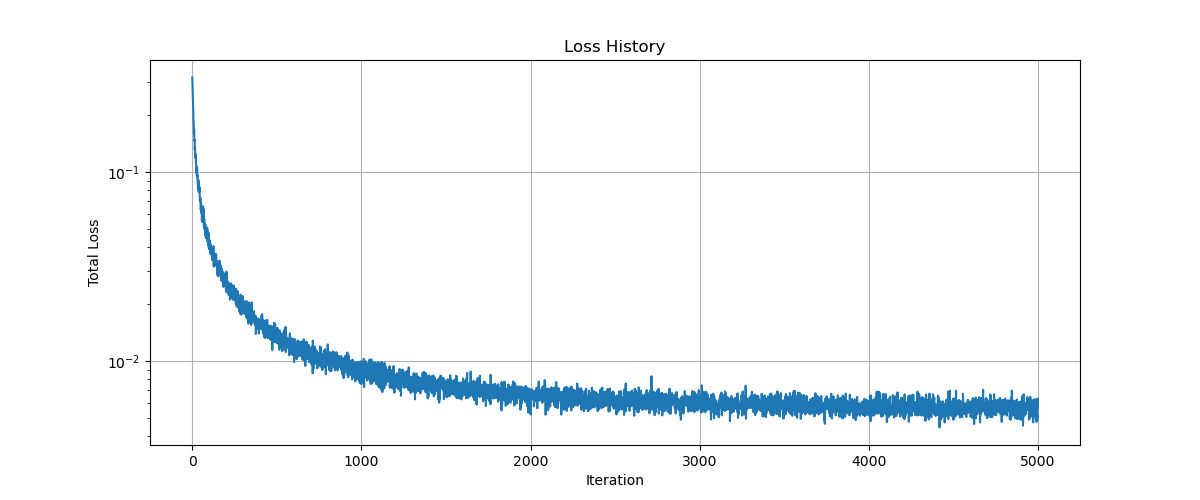
\includegraphics[width=0.8\linewidth]{lossgenf316features.png}
	\caption{Training loss for the generator with 16 nonlinear features.}
	\label{fig:loss_f3_16}
\end{figure}



\end{document}
